% !TeX root = ../main.tex
\chapter{仿真实验}
仿真实验分为三步,首先在Matlab中基于s-function和simulink仿真,验证控制算法的性能;然后在ros框架下,基于PX4固件,修改其运动控制部分的代码,在gazebo中进行软件在环仿真(SITL,software in the loop);接着,将修改后的PX4固件烧写到pixhawk飞控板中,进行硬件在环仿真(HITL,hardware in the loop),而这个版本的固件也可以直接用于后续的实机实验。
\section{Matlab仿真}
我们在Simulink环境下构建了一个综合仿真模型,该模型不仅包含了刚体动力学和电机动态,还通过s-function实现了姿态环和位置环分离的双环控制器设计。这种设计使得后续的数据分析和研究工作能够更为便捷、高效。

为了能直观地体现性能,我们设计了一个“8”字型轨迹,如图\ref{fig:8}:
$$x_d = \begin{matrix}[3\sin(\frac{t}{2}), & 3\cos(\frac{t}{2})\sin(\frac{t}{3}), &-0.1t]\end{matrix}
\quad
\psi_d=0.01t$$

\begin{figure}[!h]
  \centering
  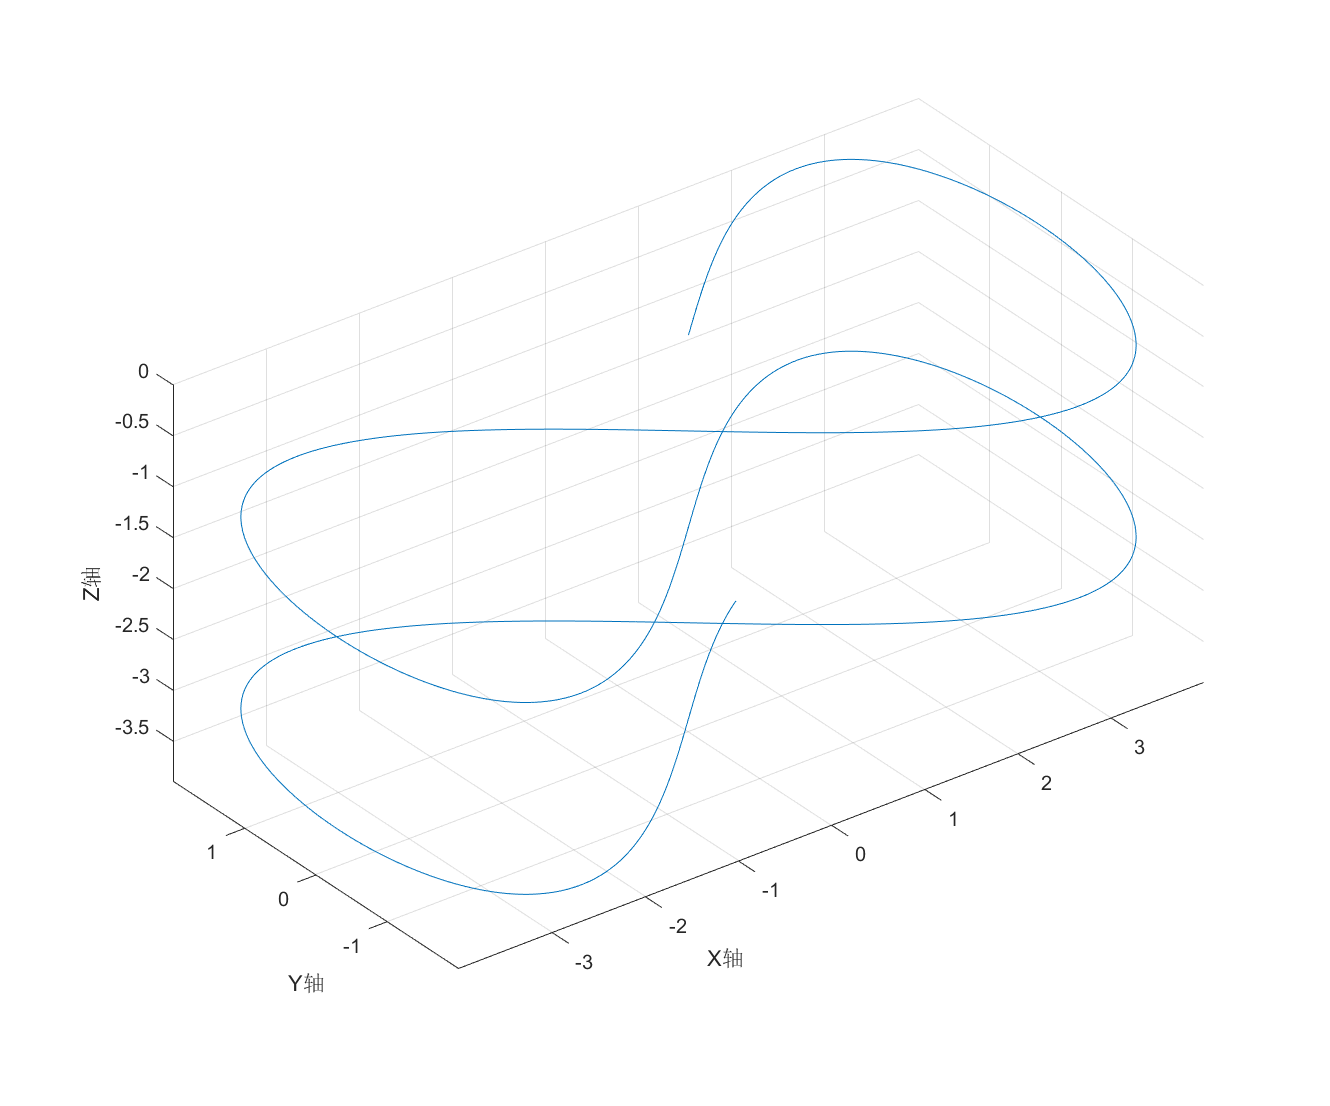
\includegraphics[width=0.5\textwidth]{88.png}
  \caption{高度匀速上升的“8”字型轨迹(北-东-地坐标系下,地面以上Z轴为负数)}
  \label{fig:8}
\end{figure}

为了全面体现控制算法的跟踪性能,我们并没有对轨迹做特殊的平滑处理,轨迹的导数存在间断点使得高阶导数无穷大,这可以考验无人机在现实中的抗扰性能。为了模拟起飞和悬停,第一秒内轨迹保持在原点不动,否则仿真就会等同在空中释放电机无转速的无人机。


  无人机的刚体动力学部分由simulink中自带的“6DOF block”解决,避免了$SO(3)$群差分近似后单位化的困难。该模块会对外部输入的力和力矩做出反应,返回所需的速度、位置、姿态、角速度等信息。

  电机部分,转速的动态由一阶惯性环节表示,根据所选电机型号时间常数$\tau=0.01s$。
  姿态控制器和位置控制器分开由两个s-function实现,重力由单独的模块输入到“6DOF block”。
  \begin{figure}[!h]
    \centering
    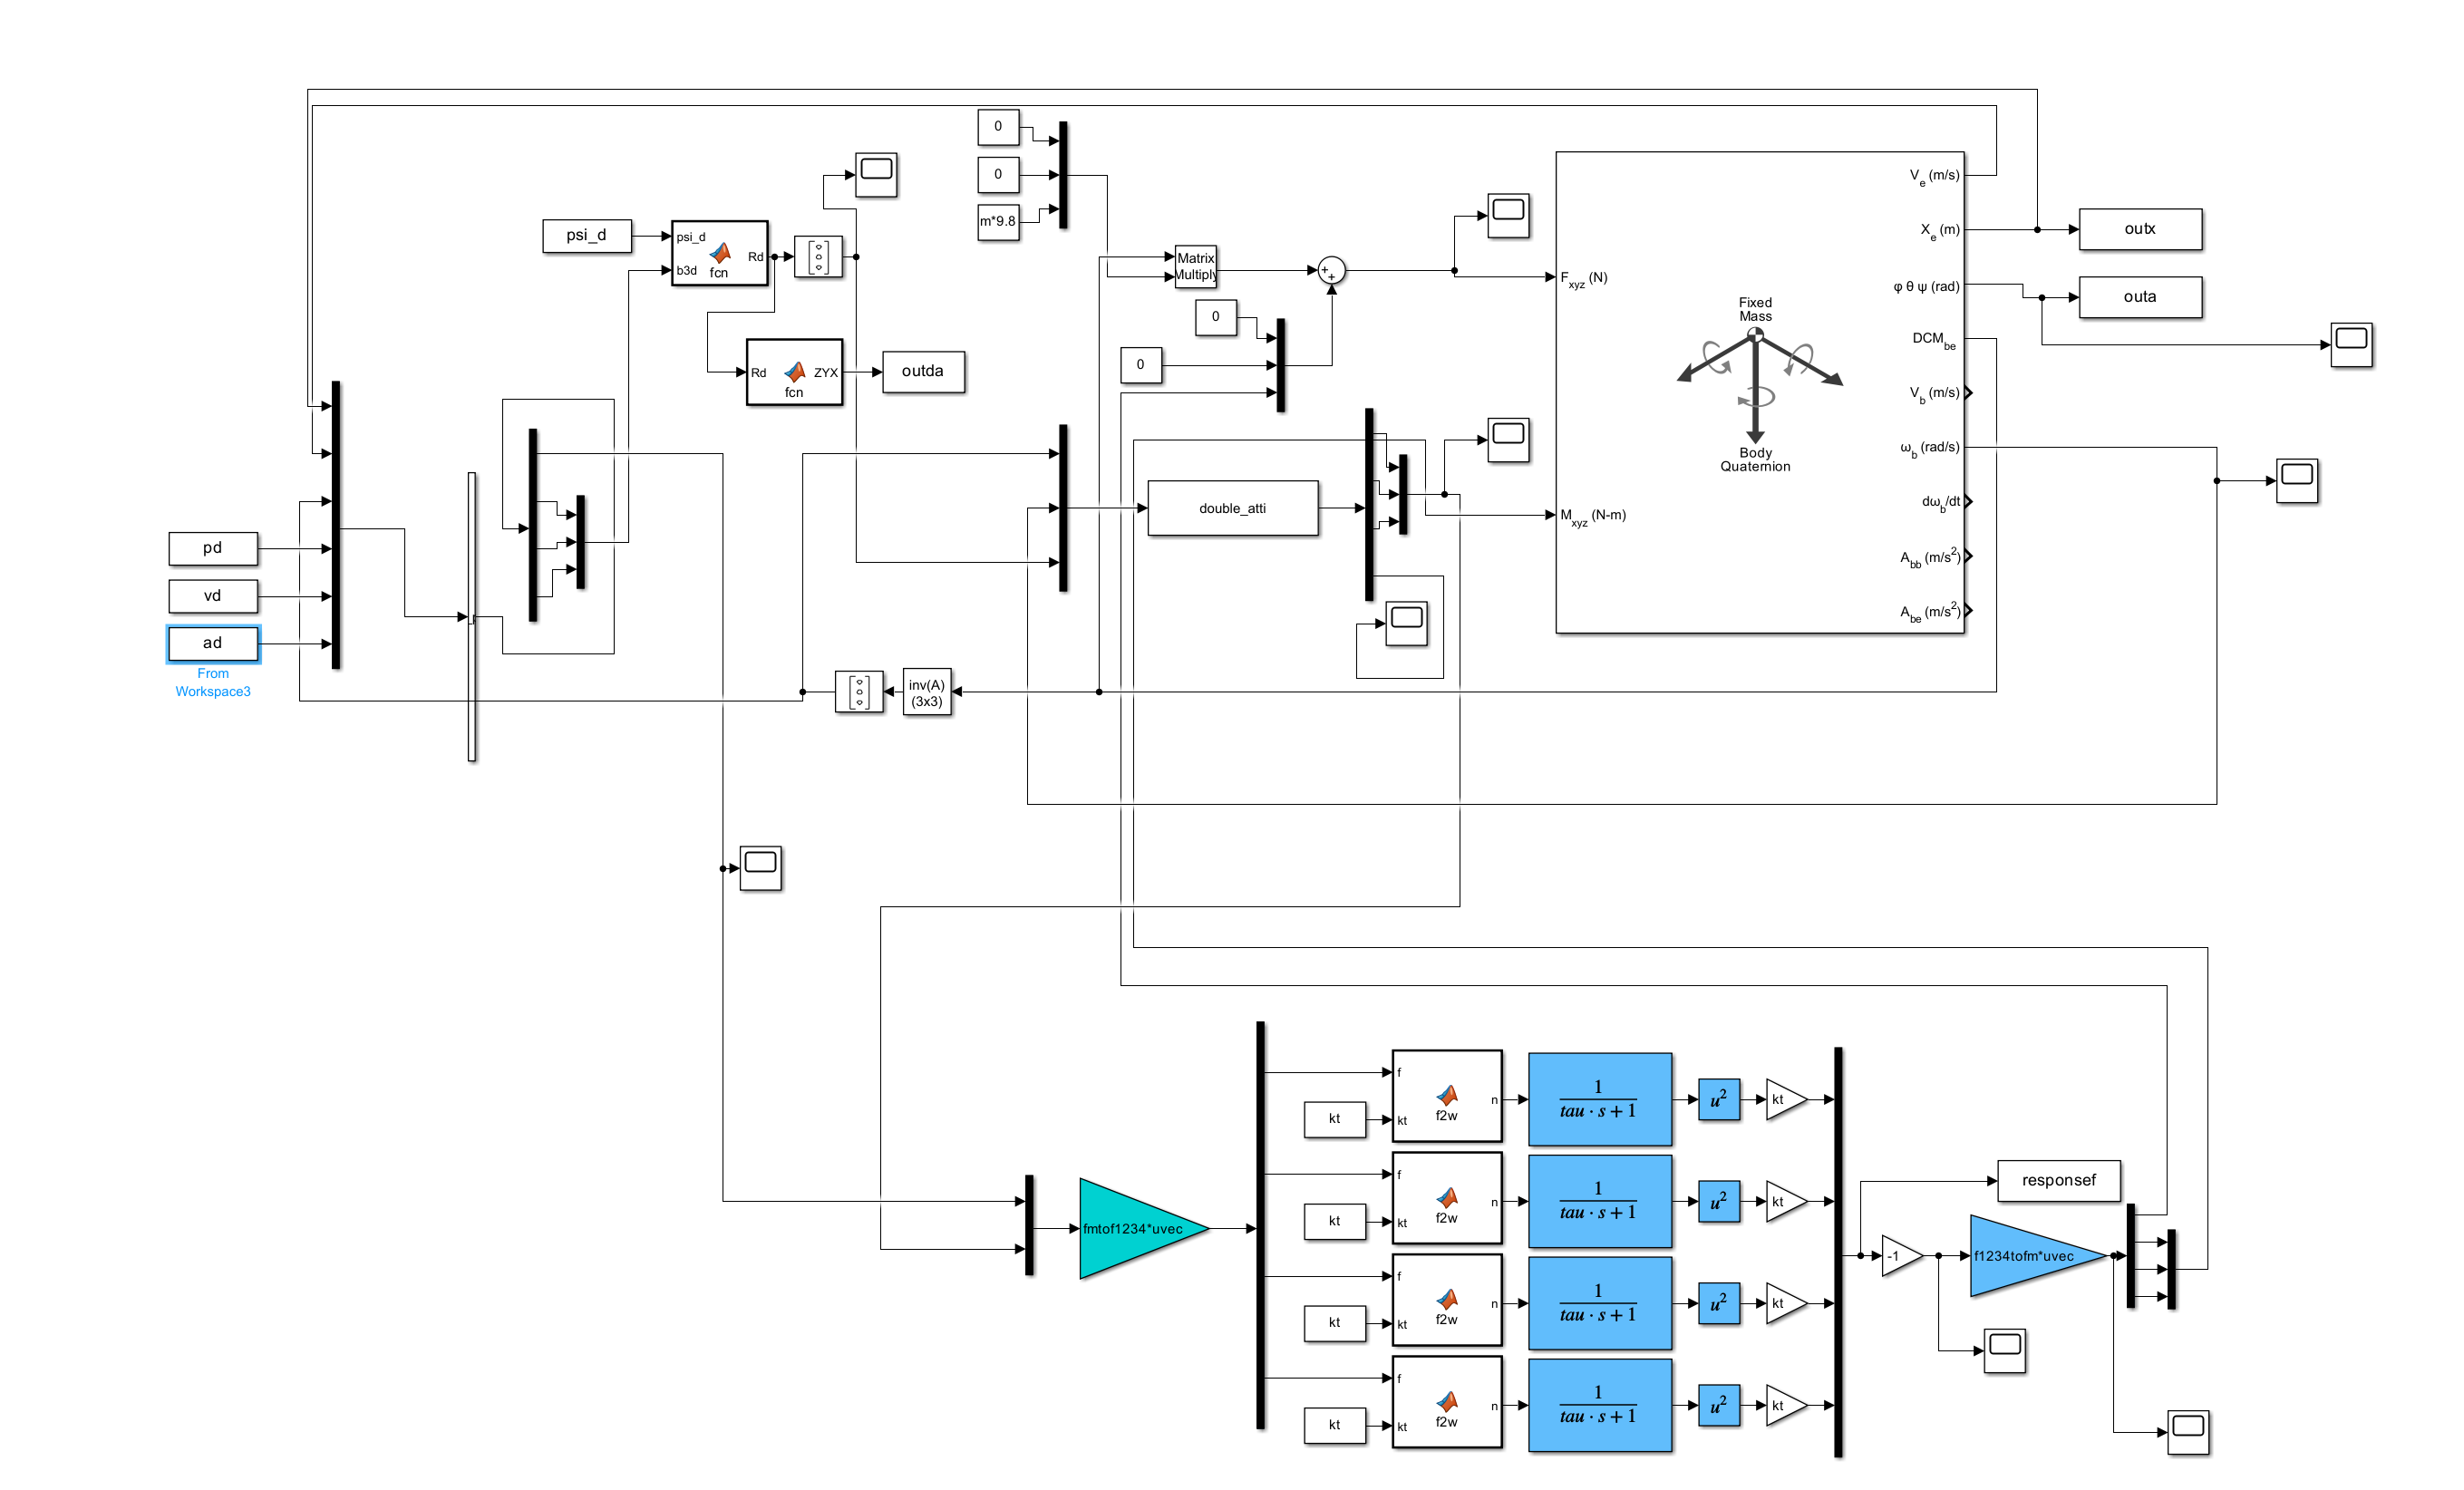
\includegraphics[width=0.9\textwidth]{sim.png}
    \caption{simulink仿真连线图}
    \label{fig:sim}
  \end{figure}

  四旋翼无人机的参数由测量和理论计算共同得到:
  $$m=0.8kg \quad d=0.125m \quad J=\begin{bmatrix}
    0.0024   &      0  &       0\\
    0 &   0.0025      &   0\\
    0  &       0   & 0.0041
  \end{bmatrix}kg m^2$$

  电机参数由厂家数据得到:
  $$k_t=2.03\times 10^{-8} \quad 
  \tau=0.01s \quad
  c_{\tau f}=8\times 10^{-3}$$

  选择替补姿态控制律:
  $$k_R=0.881 \quad k_\omega=0.254$$

  由于位置环和姿态环补偿后得到的线性系统A矩阵完全一致,因此选择相同的LQR权重矩阵:
  $$Q=\begin{bmatrix}
    3&0&0&0&0&0\\
    0&3&0&0&0&0\\
    0&0&3&0&0&0\\
    0&0&0&1&0&0\\
    0&0&0&0&1&0\\
    0&0&0&0&0&1\\
  \end{bmatrix} \quad R=\begin{bmatrix}
    0.1 &0 &0\\
    0 &0.1 &0\\
    0 &0 &0.1\\
  \end{bmatrix}$$

  初始位姿:
  $$x(0)=[0,0,0],\quad v(0)=[0,0,0]$$
  $$R(0)=I , \quad \omega(0)=[0,0,0]$$

  按照上述参数,在matlab中用0.005s的控制周期运行仿真,得到结果如图\ref{fig:result-x},\ref{fig:result-angle},\ref{fig:result-f}:
  \begin{figure}[h]
    \centering
    \begin{minipage}[c]{0.33\textwidth}
      \centering
      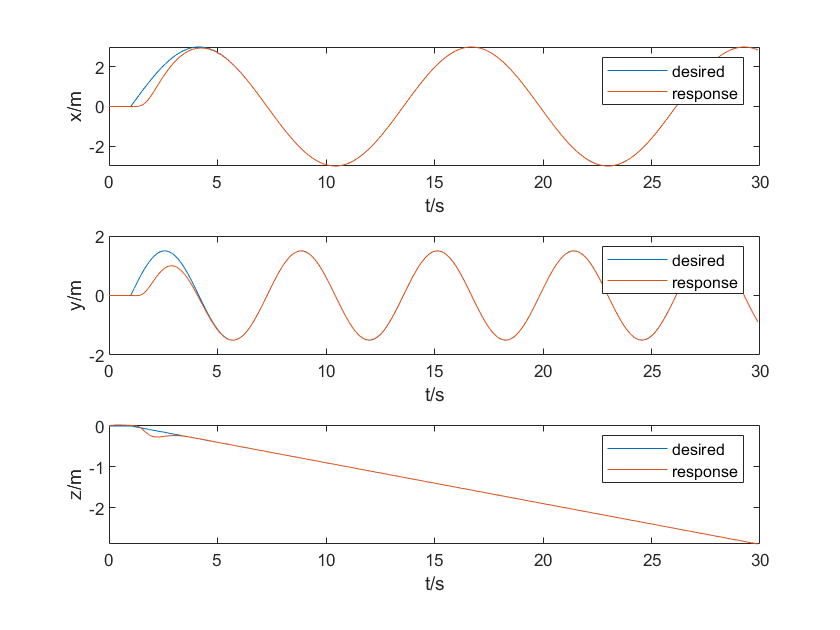
\includegraphics[width=0.95\linewidth]{result-x.png}
      \caption{位置跟踪效果}
      \label{fig:result-x}
    \end{minipage} \hfill
    \begin{minipage}[c]{0.33\textwidth}
      \centering
      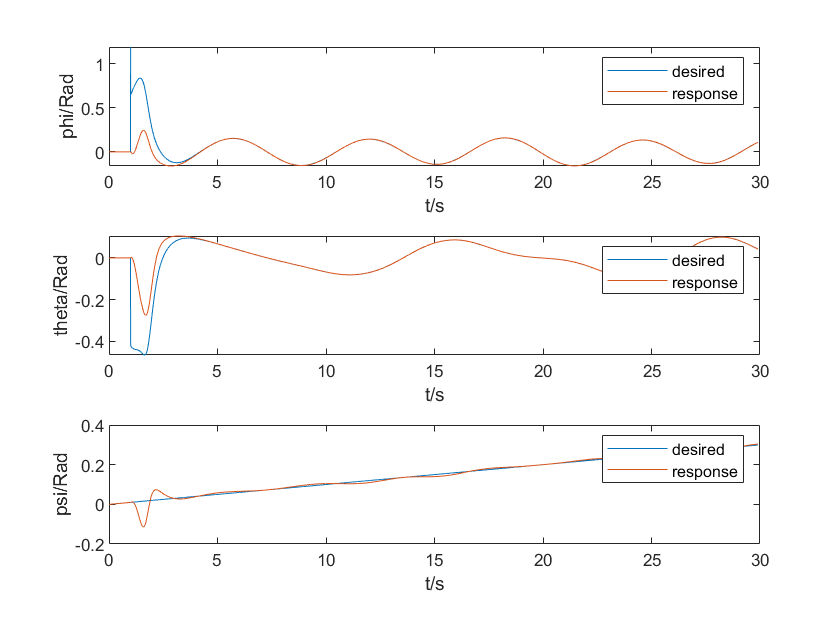
\includegraphics[width=0.95\linewidth]{result-angle.png}
      \caption{角度跟踪效果}
      \label{fig:result-angle}
    \end{minipage}\hfill
      \begin{minipage}[c]{0.33\textwidth}
        \centering
        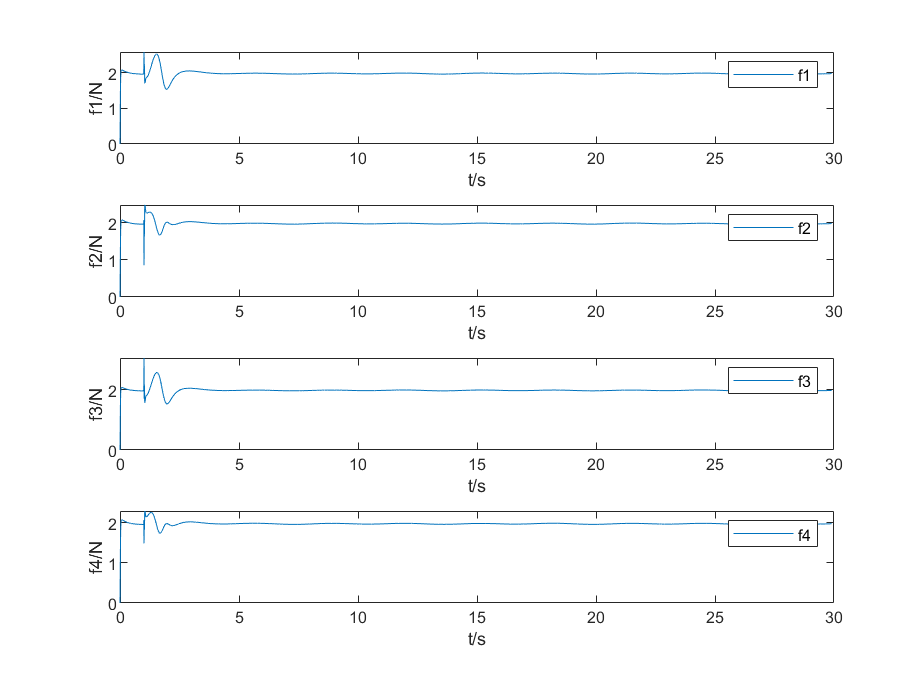
\includegraphics[width=0.95\linewidth]{result-f.png}
        \caption{四个电机输出的力}
        \label{fig:result-f}
    \end{minipage}
    \end{figure}

  从以上图中可以看到本控制算法可以很好地跟踪这种有较大姿态机动的轨迹,只是由于轨迹在起始时存在阶跃,导致无人机在阶跃处需要一定的动态过程才能跟踪上。但是在实际的飞行任务中,在轨迹规划层面就需要对轨迹做光滑处理。为了避免出现执行器饱和的情况,在仿真中我们根据无人机的实际情况和电机所能输出的最大升力,设置了控制器输出力和力矩的上限。

  \pagebreak
  
  三维空间下的轨迹跟踪情况如图\ref{fig:result-3d}

  可以看到在起始的阶跃之后,跟踪效果都十分完美,为了量化地展示跟踪效果,我们提出了平均距离误差和平均偏航角误差:
  $$e_d=\frac{\sum_0^{T}||x-x_d||}{T} \quad e_\psi=e_d=\frac{\sum_0^{T}|\psi-\psi_d|}{T}$$

  误差曲线如图\ref{fig:result-e}
 

  \begin{figure}[h]
    \centering
       \begin{minipage}[c]{0.45\textwidth}
        \centering
        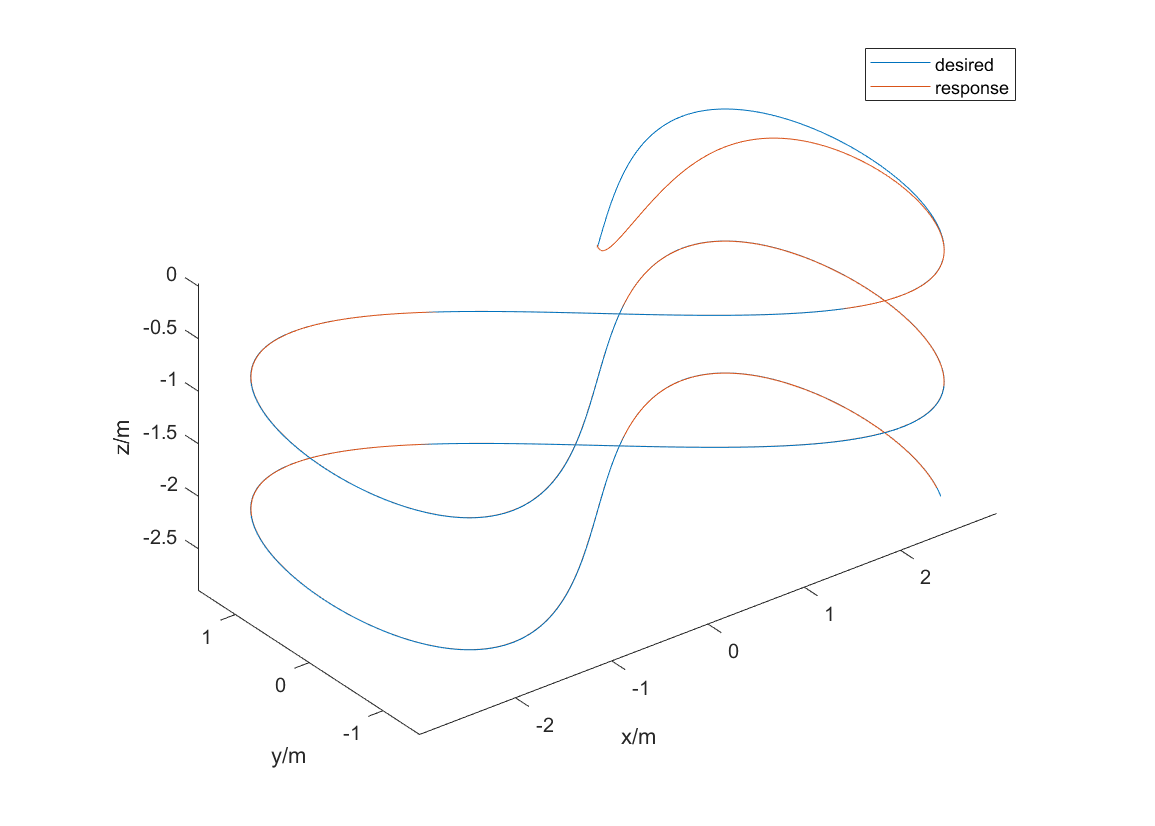
\includegraphics[width=0.9\textwidth]{result-3d.png}
        \caption{三维空间下的轨迹跟踪情况}
        \label{fig:result-3d}
     \end{minipage}%
       \begin{minipage}[c]{0.45\textwidth}
        \centering
        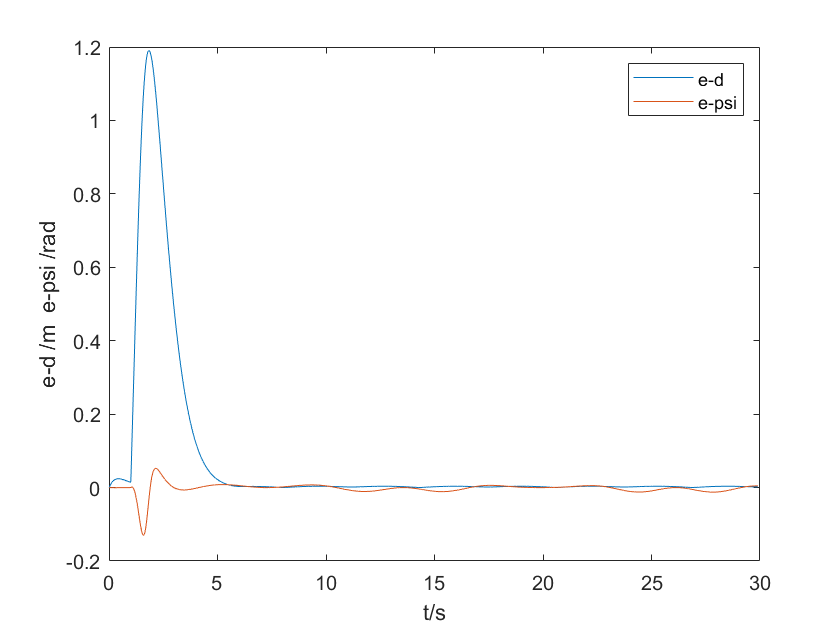
\includegraphics[width=0.9\textwidth]{result-e.png}
        \caption{平均距离误差和平均偏航角误差}
        \label{fig:result-e}
     \end{minipage}
   \end{figure}

   为了体现本控制方法的优越性,设置对照组,与\cite{Lee2010}中也就是上文所说的替补姿态控制律对比(位置环相同):
   
  \begin{figure}[h]
    \centering
    \begin{minipage}[c]{0.33\textwidth}
      \centering
      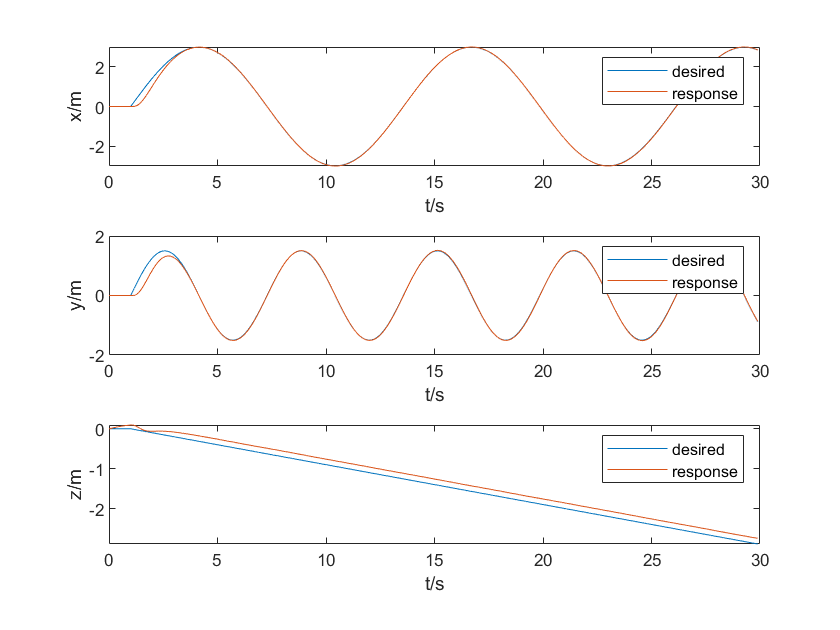
\includegraphics[width=0.95\linewidth]{com-x.png}
      \caption{对照组位置跟踪效果}
      \label{fig:com-x}
    \end{minipage} \hfill
    \begin{minipage}[c]{0.33\textwidth}
      \centering
      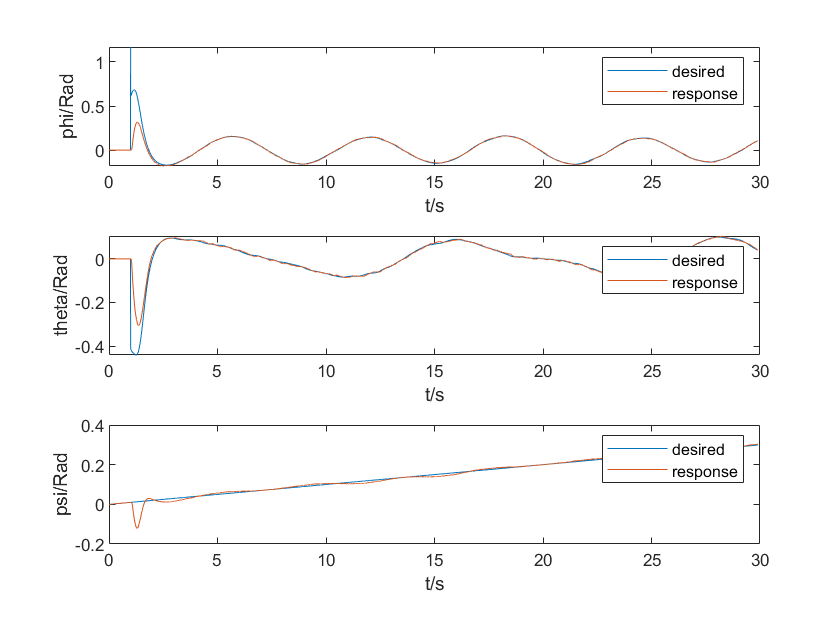
\includegraphics[width=0.95\linewidth]{com-angle.png}
      \caption{对照组角度跟踪效果}
      \label{fig:com-angle}
    \end{minipage}\hfill
      \begin{minipage}[c]{0.33\textwidth}
        \centering
        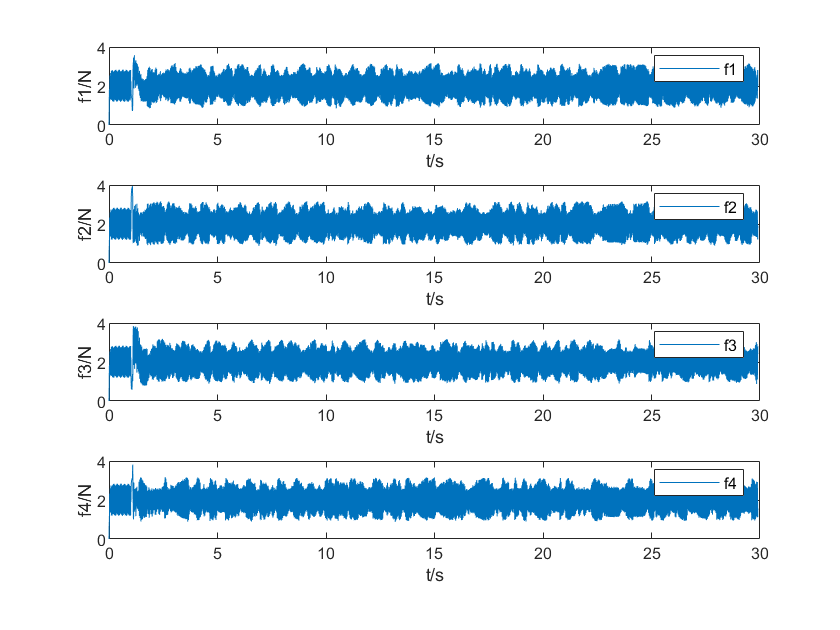
\includegraphics[width=0.95\linewidth]{com-f.png}
        \caption{对照组四个电机输出的力}
        \label{fig:com-f}
    \end{minipage}
    \end{figure}

    \begin{figure}[h]
      \centering
         \begin{minipage}[c]{0.45\textwidth}
          \centering
          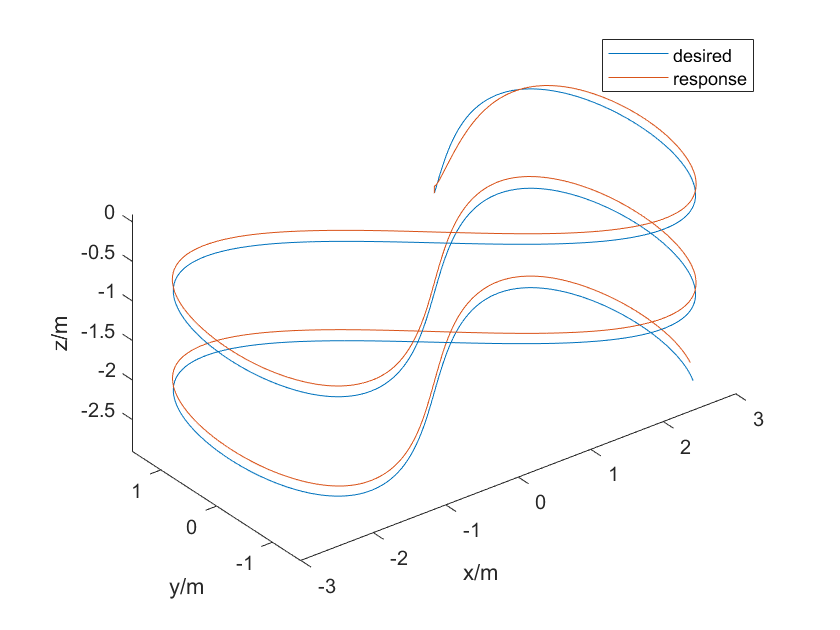
\includegraphics[width=0.9\textwidth]{com-3d.png}
          \caption{对照组三维空间下的轨迹跟踪情况}
          \label{fig:com-3d}
       \end{minipage}%
         \begin{minipage}[c]{0.45\textwidth}
          \centering
          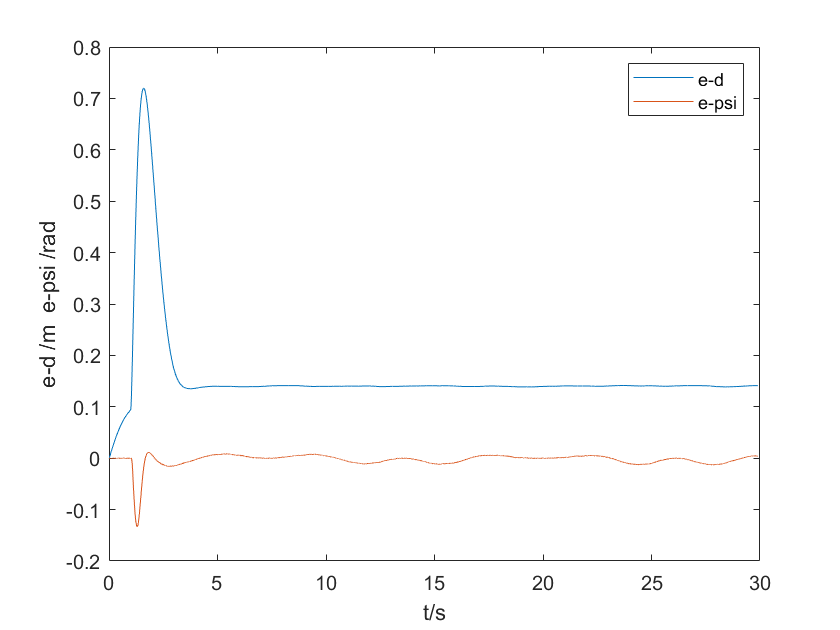
\includegraphics[width=0.9\textwidth]{com-e.png}
          \caption{对照组平均距离误差和平均偏航角误差}
          \label{fig:com-e}
       \end{minipage}
     \end{figure}

     从图\ref{fig:com-3d}中可以直观地看到其跟踪始终有误差未能弥合,在阶跃处同样需要一个动态过程。图\ref{fig:com-f}显示,其推力始终有剧烈抖动,这有可能是因为姿态环的参数调节欠缺。但这正体现了HOFA方法的优越性,相比于对照组的参数调节缺乏理论指导,只能根据经验多次尝试,HOFA方法能将非线性部分全部补偿掉,留下的线性系统对LQR参数并不敏感,权重矩阵并不需要精细地多次调解就能取得很好的控制效果。
     \begin{table}
      \centering
      \begin{tabular}{ccc}
          \toprule
          & 平均距离误差 & 平均偏航角误差 \\
          \midrule
          HOFA方法 & 0.0692 & 0.0072 \\
          对照组 & 0.1580 & 0.0065 \\
          \bottomrule
      \end{tabular}
      \caption{HOFA方法与对照组的平均误差对比}
  \end{table}

  量化的误差指标同样显示,在位置跟踪上,HOFA大幅领先于对照组。在偏航角误差的指标上,有小幅落后,但两者的误差都已经很小。

\section{软件在环仿真}
Matlab仿真只是初步验证了HOFA方法的有效性,既没有考虑实际的飞控固件中异步的采样周期、进程管理等因素,也没有考虑内部和外部传感器信息融合的因素。而在ros+gazebo下的软件在环仿真会考虑以上因素,进一步贴近实际情况。

首先配置环境,由于当前ros2适配的各种依赖库包括PX4的版本都还在不停迭代,因此目前还是选择更为稳定、资料更多的ros1。在ubuntu20.04中安装ros1 noetic以及配套的mavros和gazebo11 classic,然后从GitHub上clone最近的发行版PX4 v1.14.0,注意要使用递归将所有子项目克隆下来。

git clone -b v1.14.0 https://github.com/PX4/PX4-Autopilot.git --recursive

然后运行Tools/setup/ubuntu.sh,解决编译的依赖。最后运行软件在环仿真命令:make px4_sitl gazebo-classic。运行成功后会进入gazebo仿真界面,打开QGC会自动连接地面站,在地面站中可以方便地看到回传的位姿信息并且发布起飞和指点飞行命令。